\chapter{Alternative Classifier Structures} 
\label{app:2bmodel}

In this appendix the architectures presented in \secref{2bmodels} are shown. As previously said these architectures features 2 separate convolutional branches receiving as input the output of a splitting layer. 
In \figref{fig:2bap_model} the variant with implemented average pooling layers is shown, while the one with no pooling layers is shown in \figref{fig:2bnp_model}.

As for the ones shown in \figref{fig:1b_model} and \figref{fig:1bnp_model} the implementation of these architectures was perfoemed using the Functional API of the Keras framework.

All the main features and hyperparameters are the same as the ones for the architectures described in \chapref{chap5}, namely:
\begin{itemize}
    \item L2 loss function in each layer
    \item ADAM optimizer
    \item Dropout rate of 30\% after the dense layer in the communication protocol branch
    \item Zero padding technique implemented in the architecture without pooling layers
    \item ELU activation function after each hidden layer
    \item Softmax activation function for the last layer
\end{itemize}

\begin{figure}
   % \centering
\hspace{-2cm}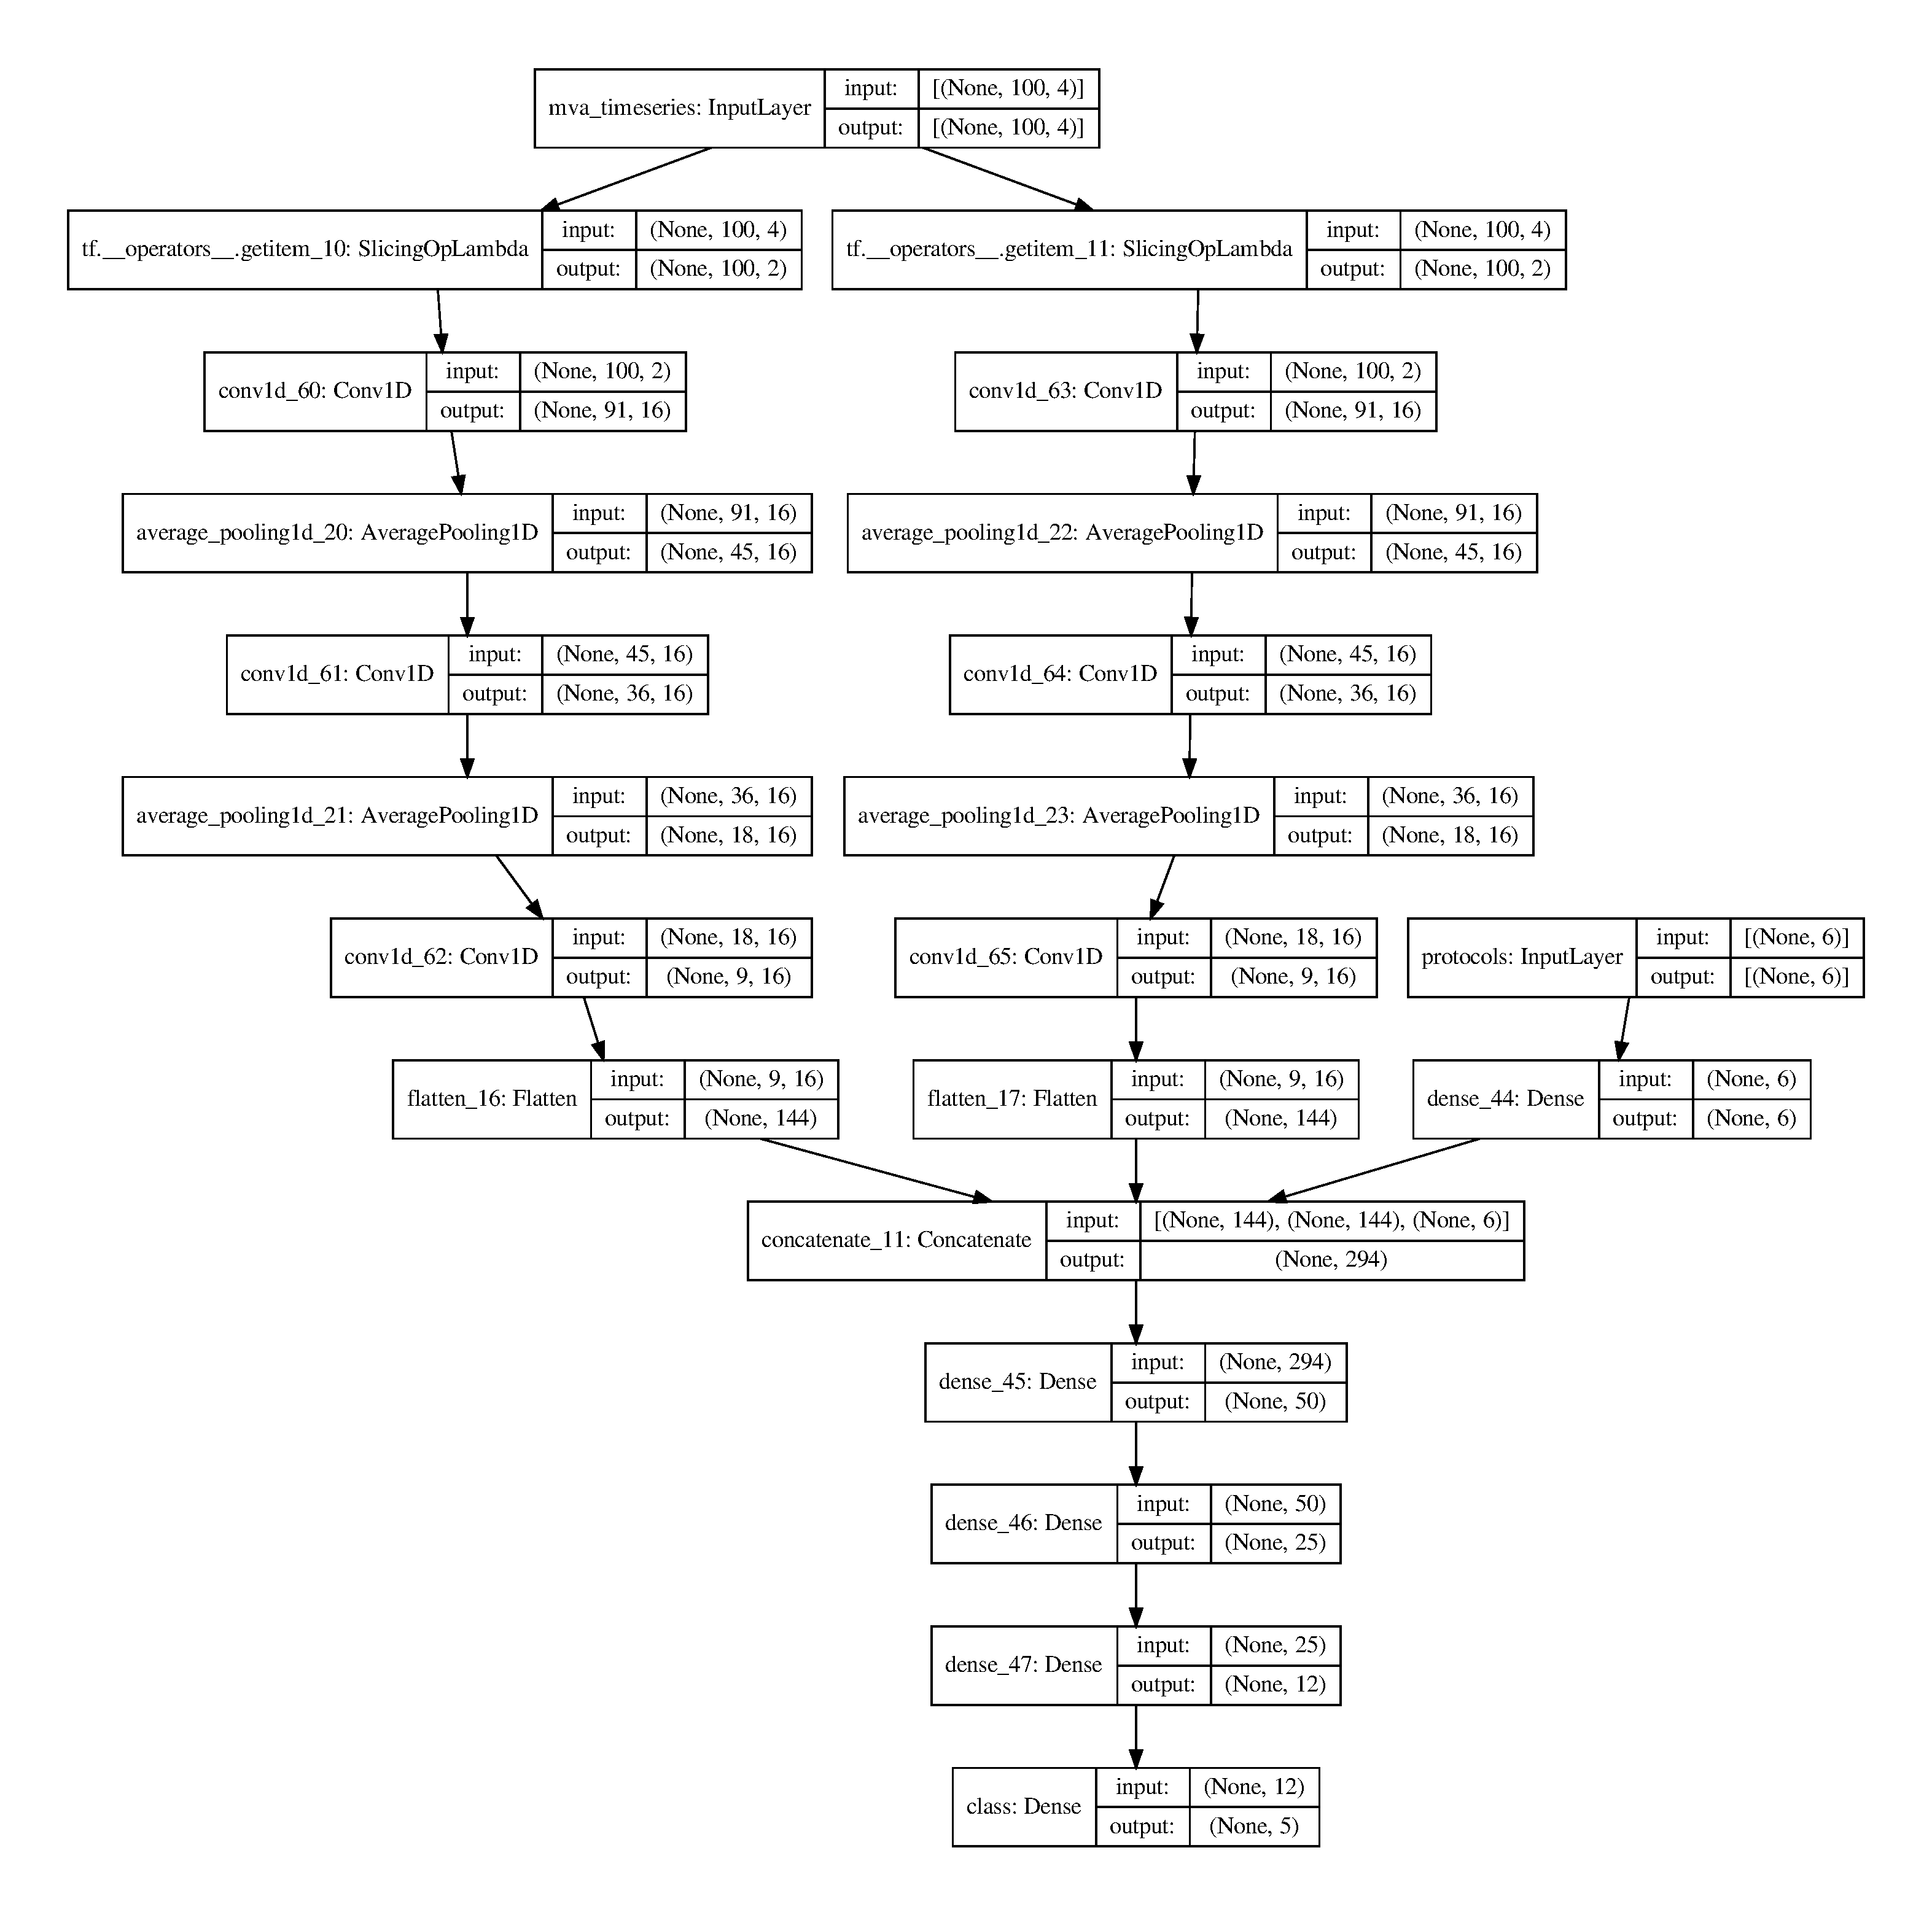
\includegraphics[width=1.3\textwidth]{images/models/model_2bap.pdf}
\caption{{Structure of the proposed classifier 1B\_NP architecture. The name indicates the presence of two convolutional branch and the absence of pooling layers.}}    \label{fig:2bap_model}
\end{figure}




\begin{figure}
  %  \centering
    \hspace{-2cm}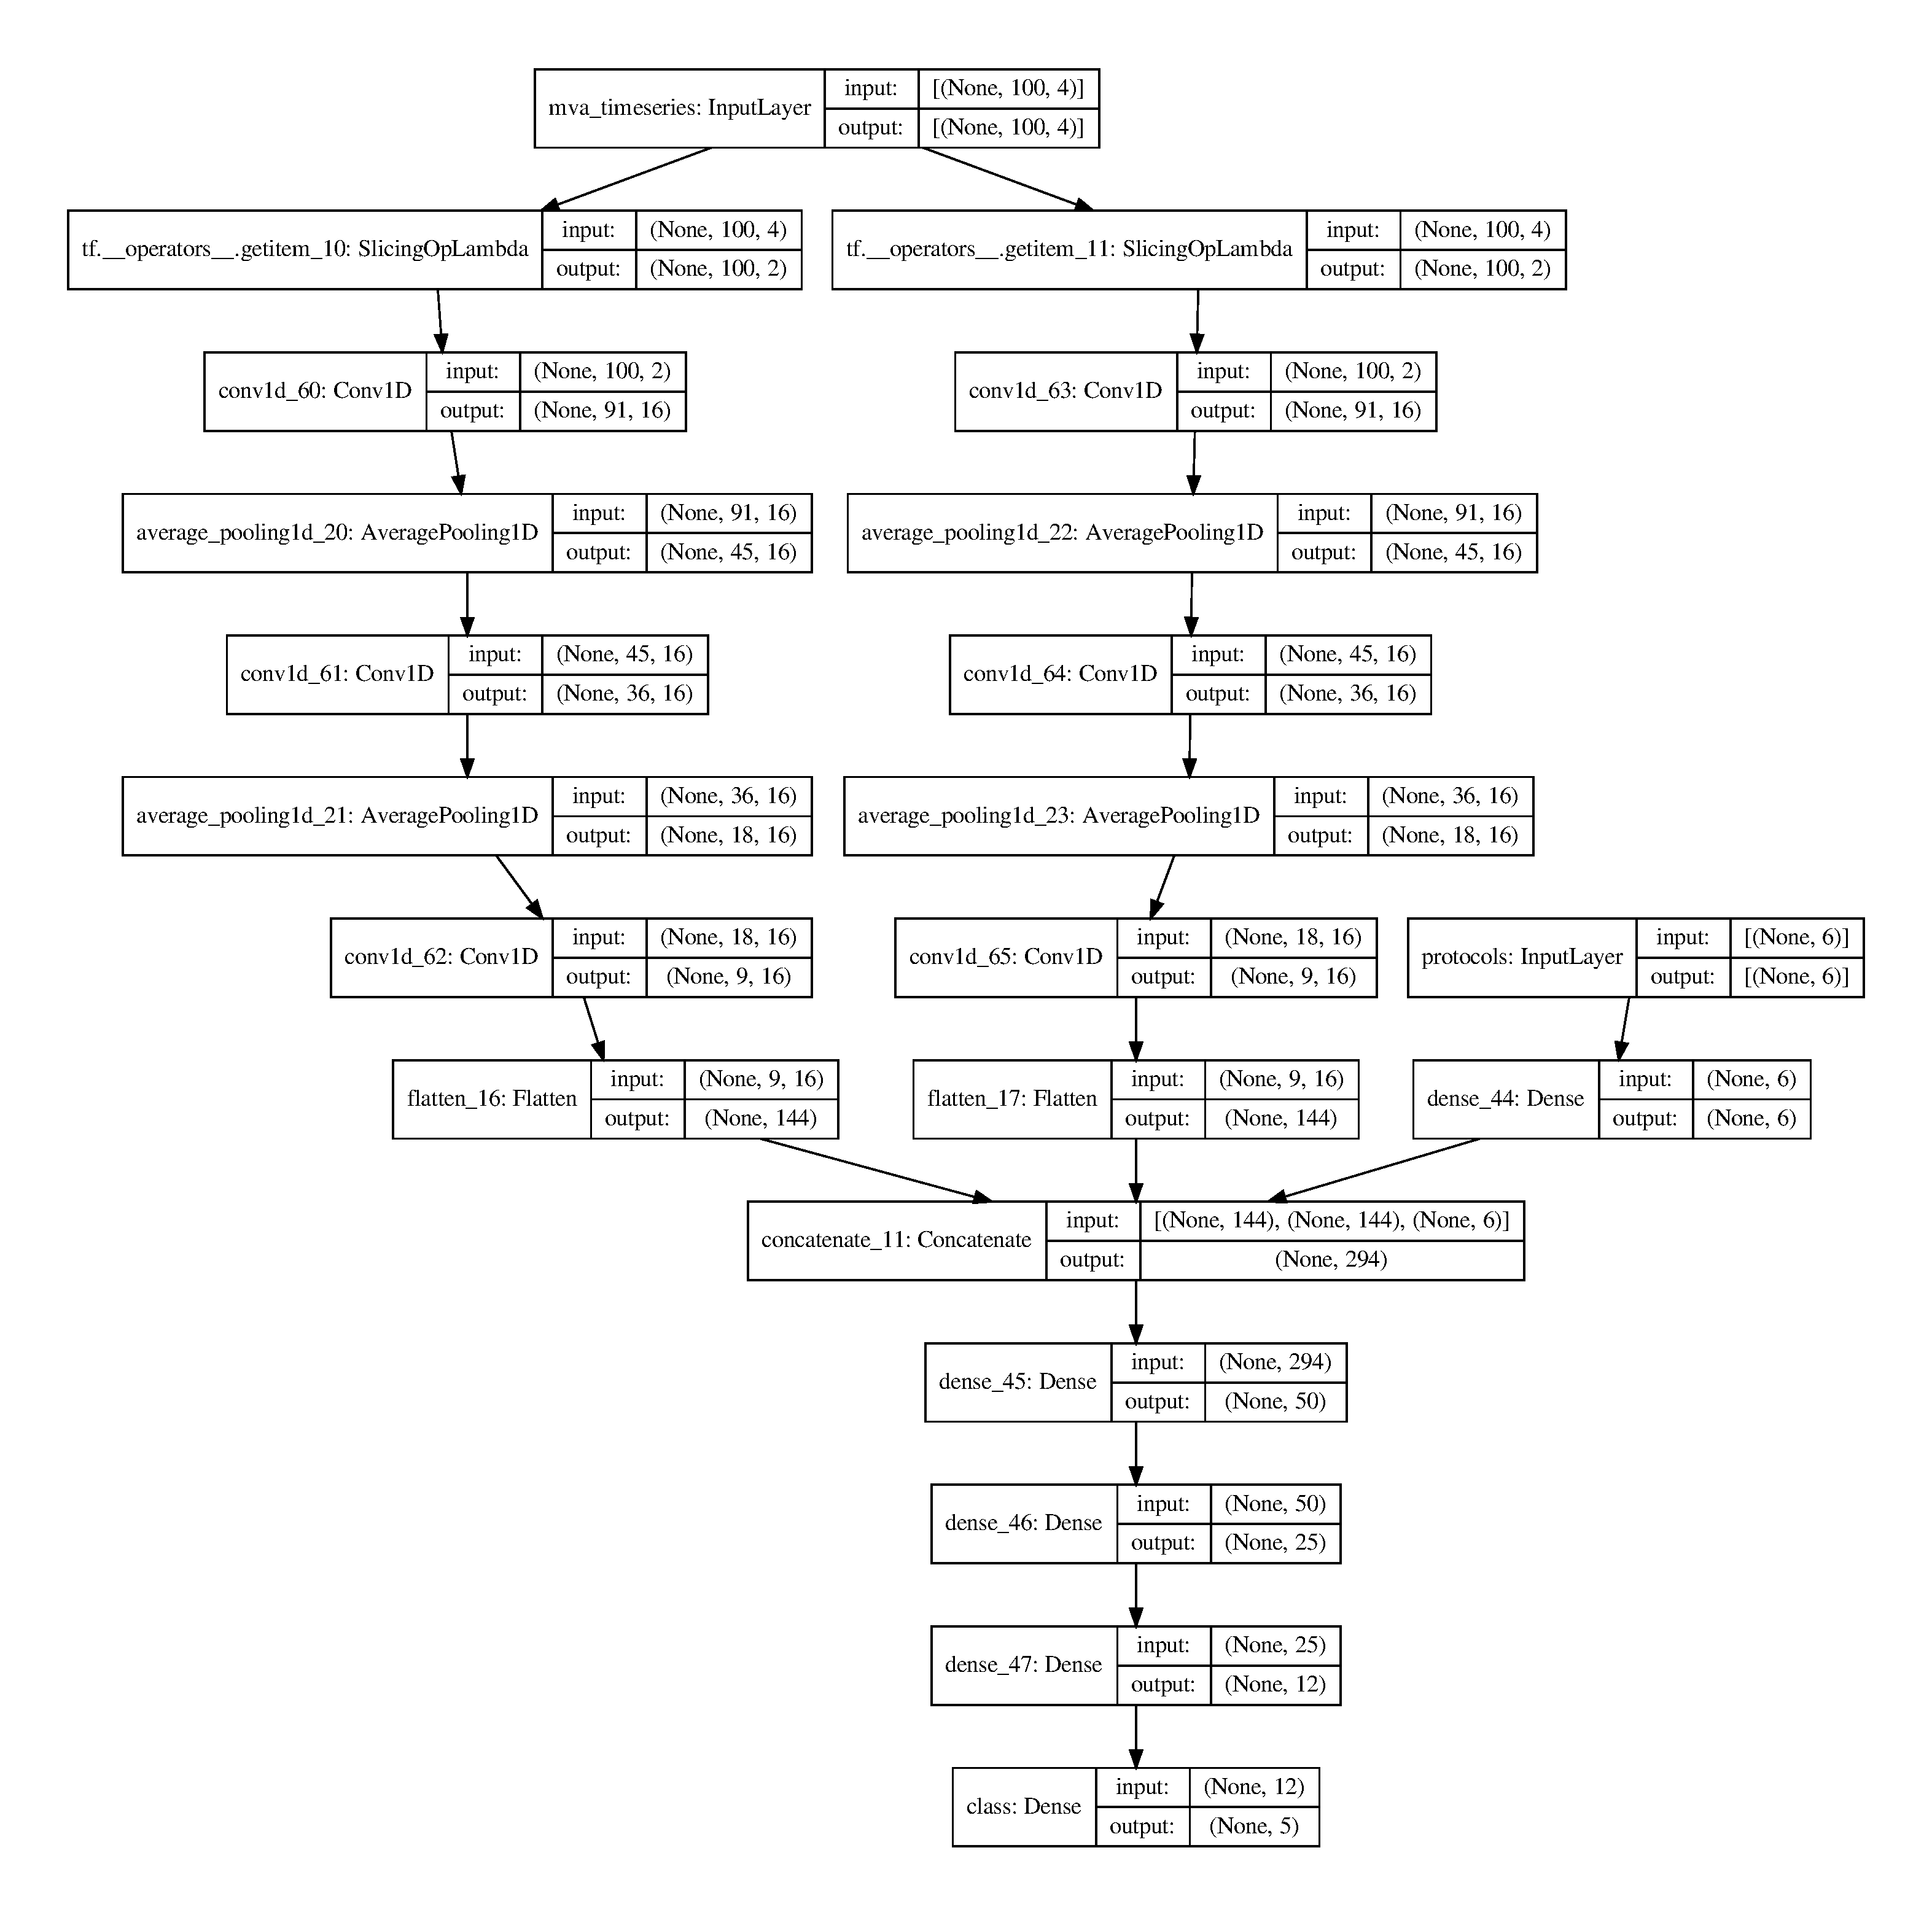
\includegraphics[width=1.3\textwidth]{images/models/model_2bnp.pdf}
\caption{{Structure of the proposed classifier 1B\_NP architecture. The name indicates the presence of two convolutional branch and the absence of pooling layers.}}    \label{fig:2bnp_model}
\end{figure}




\chapter{Appendix B}
\label{app:lb_bonus_res}

In this appendix additional plots for the analysis of the lookback values, discussed in \secref{res_lb} are shown. The plots show the evolution of the model accuracy and loss function during the training of the 1B\_NP architecture. The training is performed using time series for the 4SICS dataset with different lookback $L$ values during the preprocessing step. 

\begin{figure}[!h]
    \centering
    \begin{minipage}[c]{0.49\textwidth}
        \vspace{0pt}
        \centering
        \subfloat[Loss function]{
        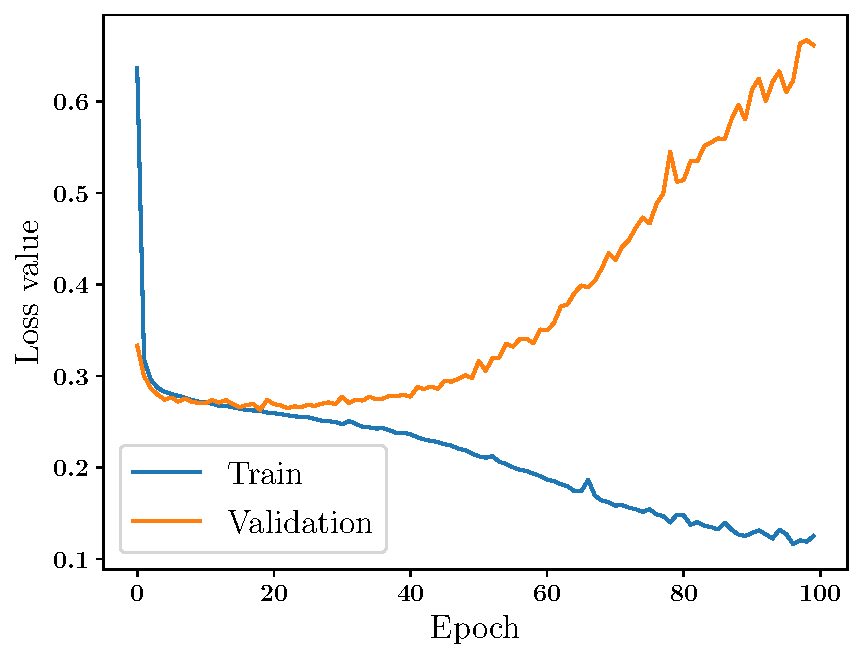
\includegraphics[width=\textwidth]{images/results/LB_test_25_20210620-165709__type_1branch_no_pool__st_scale_sub__lb_10__act_elu__nf_16__ks_10__nn_50__l2_1e-05__bs_200__ep_100__loss.pdf}
            \label{fig:lb_10_loss}
        }
    \end{minipage}%
    \hfill%
    \begin{minipage}[c]{0.49\textwidth}
        \vspace{0pt}
        \centering
        \subfloat[Model accuracy]{
        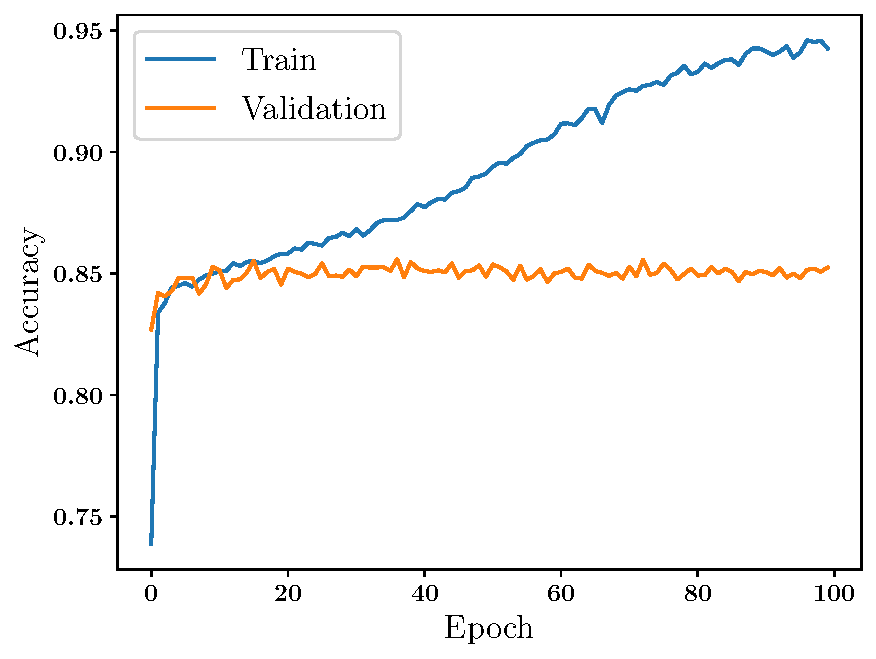
\includegraphics[width=\textwidth]{images/results/LB_test_25_20210620-165709__type_1branch_no_pool__st_scale_sub__lb_10__act_elu__nf_16__ks_10__nn_50__l2_1e-05__bs_200__ep_100___accuracy.pdf}
            \label{fig:lb_10_acc}
        }
    \end{minipage}

    \caption{Loss function and model accuracy during training with $L=15$.}
    \label{fig:res_lb_val}
\end{figure}

\begin{figure}[!h]
    \centering
    \begin{minipage}[c]{0.49\textwidth}
        \vspace{0pt}
        \centering
        \subfloat[Loss function with lookback $L=25$]{
        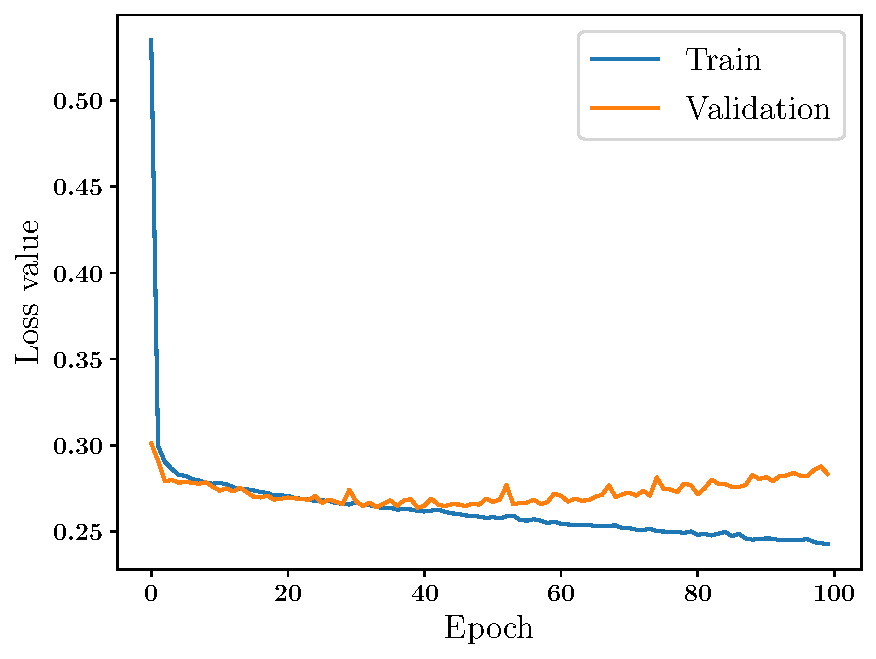
\includegraphics[width=\textwidth]{images/results/LB_test_15_20210620-165532__type_1branch_no_pool__st_scale_sub__lb_5__act_elu__nf_16__ks_10__nn_50__l2_1e-05__bs_200__ep_100__loss.pdf}
            \label{fig:lb_10_loss}
        }
    \end{minipage}%
    \hfill%
    \begin{minipage}[c]{0.49\textwidth}
        \vspace{0pt}
        \centering
        \subfloat[Model accuracy]{
        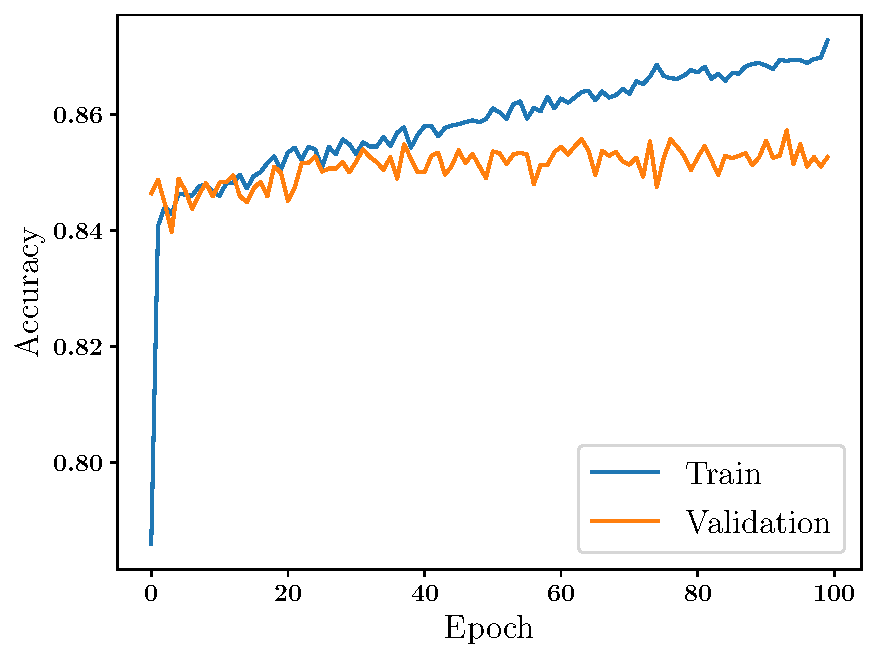
\includegraphics[width=\textwidth]{images/results/LB_test_15_20210620-165532__type_1branch_no_pool__st_scale_sub__lb_5__act_elu__nf_16__ks_10__nn_50__l2_1e-05__bs_200__ep_100___accuracy.pdf}
            \label{fig:lb_10_acc}
        }
    \end{minipage}

    \caption{Loss function and model accuracy during training with $L=25$.}
    \label{fig:res_lb_val}
\end{figure}


\begin{figure}[!h]
    \centering
    \begin{minipage}[c]{0.49\textwidth}
        \vspace{0pt}
        \centering
        \subfloat[Loss function]{
        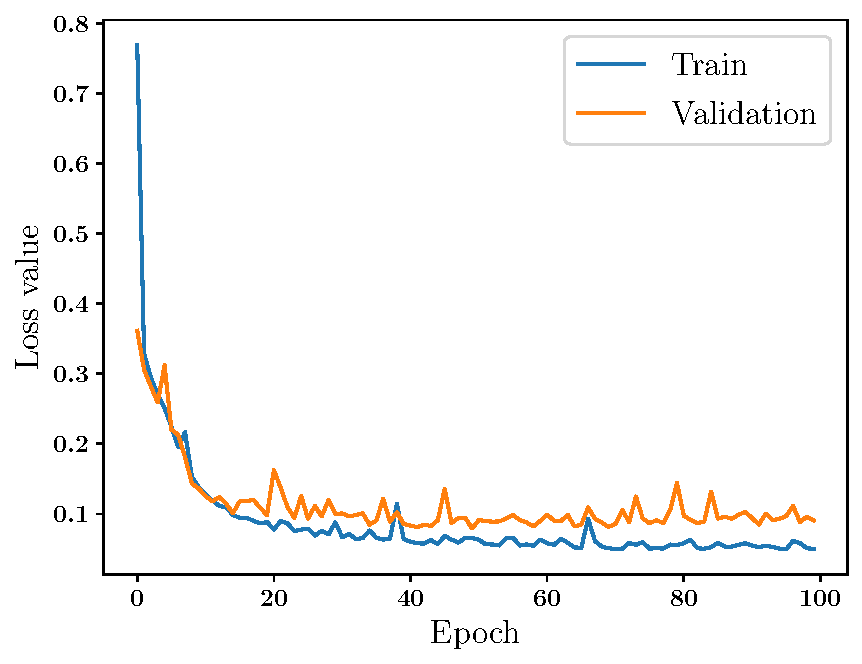
\includegraphics[width=\textwidth]{images/results/LB_test_50_20210613-181651__type_1branch_no_pool__st_scale_sub__lb_50__act_elu__nf_16__ks_10__nn_50__l2_1e-05__bs_200__ep_100__loss.pdf}
            \label{fig:lb_10_loss}
        }
    \end{minipage}%
    \hfill%
    \begin{minipage}[c]{0.49\textwidth}
        \vspace{0pt}
        \centering
        \subfloat[Model accuracy]{
        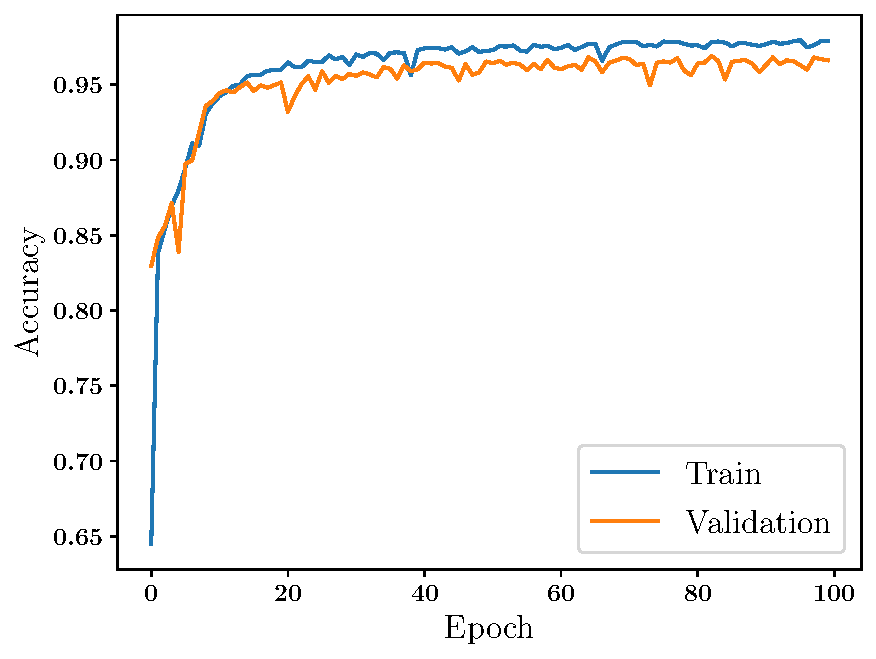
\includegraphics[width=\textwidth]{images/results/LB_test_50_20210613-181651__type_1branch_no_pool__st_scale_sub__lb_50__act_elu__nf_16__ks_10__nn_50__l2_1e-05__bs_200__ep_100___accuracy.pdf}
            \label{fig:lb_10_acc}
        }
    \end{minipage}

    \caption{Loss function and model accuracy during training with $L=35$.}
    \label{fig:res_lb_val}
\end{figure}

\begin{figure}[!h]
    \centering
    \begin{minipage}[c]{0.49\textwidth}
        \vspace{0pt}
        \centering
        \subfloat[Loss function]{
        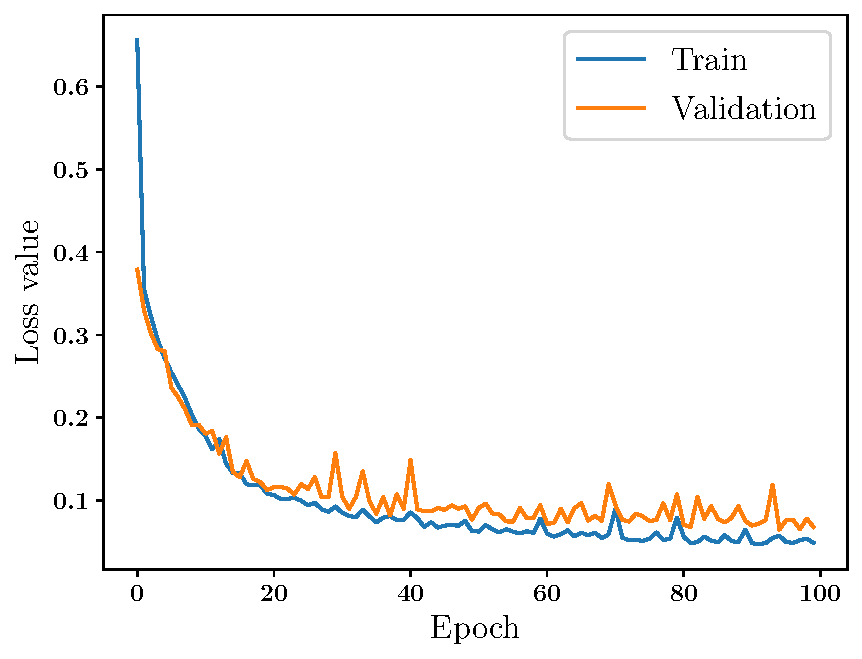
\includegraphics[width=\textwidth]{images/results/LB_test_100_20210613-180220__type_1branch__st_scale_sub__lb_100__act_elu__nf_16__ks_10__nn_50__l2_1e-05__bs_200__ep_100__loss.pdf}
            \label{fig:lb_10_loss}
        }
    \end{minipage}%
    \hfill%
    \begin{minipage}[c]{0.49\textwidth}
        \vspace{0pt}
        \centering
        \subfloat[Model accuracy]{
        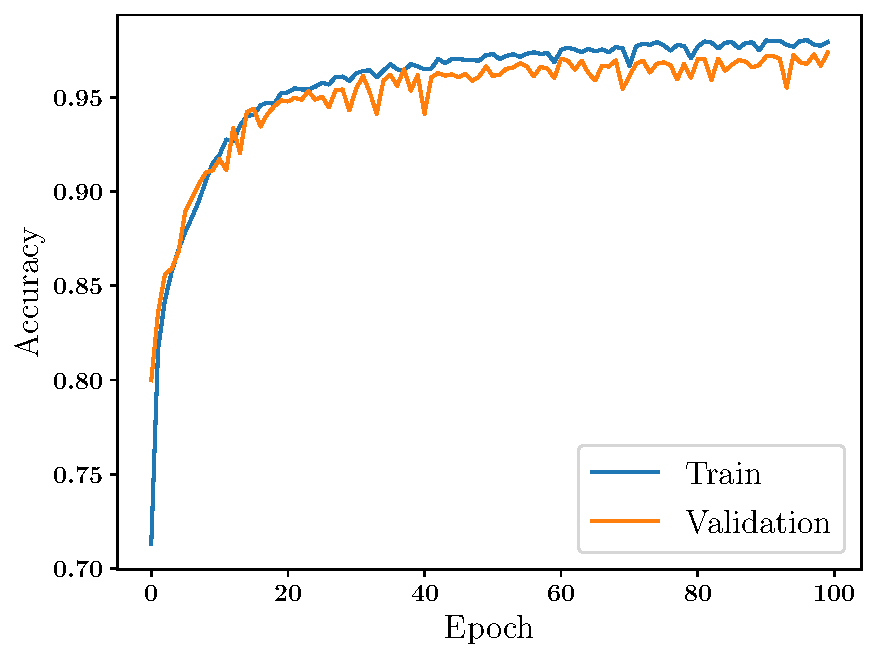
\includegraphics[width=\textwidth]{images/results/LB_test_100_20210613-180220__type_1branch__st_scale_sub__lb_100__act_elu__nf_16__ks_10__nn_50__l2_1e-05__bs_200__ep_100___accuracy.pdf}
            \label{fig:lb_10_acc}
        }
    \end{minipage}

    \caption{Loss function and model accuracy during training with $L=50$.}
    \label{fig:res_lb_val}
\end{figure}